\documentclass[11pt,a4paper]{article}
\usepackage{fontspec}
\setmainfont{TeX Gyre Pagella}
\newfontfamily\headfont{Inter}[UprightFont=*-ExtraBold,BoldFont=*-ExtraBold,Extension=.otf,Path=/usr/share/fonts/opentype/inter/]
\usepackage[a4paper,margin=2.3cm]{geometry}
\usepackage{graphicx,booktabs,float,caption,array,xcolor}
\usepackage[hidelinks]{hyperref}
\usepackage{titlesec}
\usepackage[round]{natbib}
\usepackage{setspace}
\setstretch{1.05}
\renewcommand{\topfraction}{0.9}
\renewcommand{\bottomfraction}{0.8}
\renewcommand{\textfraction}{0.1}
\renewcommand{\floatpagefraction}{0.75}
\setlength{\parindent}{0pt}
\setlength{\parskip}{0.55em}
\titleformat{\section}{\headfont\Large}{\thesection}{0.8em}{}
\titleformat{\subsection}{\headfont\large}{\thesubsection}{0.8em}{}
\captionsetup{font=small,labelfont=bf}
\urlstyle{same}
\hypersetup{pdftitle={Faith on the Map: Religion Around the World and Across the UK},pdfauthor={Tristan Hotham}}

\begin{document}
\begin{center}
{\Large\bfseries Faith on the Map\par}
\vspace{0.4em}
{\large Religion around the world and across the UK, from Pew Research Center\\estimates, the UK censuses and OpenStreetMap\par}
\vspace{1.2em}
{\large Tristan Hotham\par}
\vspace{0.3em}
{\small Independent researcher\\
ORCID: 0000-0003-4931-9349\\
DOI: \href{https://doi.org/10.5281/zenodo.23842991}{https://doi.org/10.5281/zenodo.23842991}\par}
\vspace{0.8em}
2026
\end{center}

\begin{quote}
\small
\begin{center}\textbf{Abstract}\end{center}
I bring together three open sources to describe religious affiliation around the world and across the United Kingdom, and publish them as an interactive atlas. Pew Research Center's estimates for 201 countries and territories show that between 2010 and 2020 the number of Muslims grew by 20.7\% and the religiously unaffiliated by 16.5\%, against 12.3\% for the world's population, while the Christian share fell from 30.6\% to 28.8\% and sub-Saharan Africa overtook Europe as home to the largest share of the world's Christians (30.7\% against 22.3\%). Harmonised census data for the four UK nations show Christian affiliation in England and Wales falling from 59.3\% in 2011 to 46.2\% in 2021, no religion the most common answer in 75 of 361 local authorities, a majority with no religion in Scotland (51.1\%), and a steep age gradient: 77\% of people aged 75 and over in England and Wales are Christian against 31\% of those aged 25 to 34. A series for Northern Ireland from 1861 shows Catholics outnumbering the three largest Protestant churches combined since 2001. Finally, 1,624,818 places of worship mapped in OpenStreetMap give a picture of religious landscapes and denominations, but one shaped by very uneven mapping: 77.5 mapped places per 100,000 people in North America against 7.1 in sub-Saharan Africa. The study is descriptive and makes no judgement about any religion or none.

\textbf{Keywords:} religion; religious affiliation; census; no religion; secularisation; Christianity; Islam; Northern Ireland; OpenStreetMap; places of worship; mapping
\end{quote}

\section{Introduction}
Religious affiliation is among the most widely collected and most widely discussed facts about populations, and among the hardest to measure well. National censuses ask about it in different words or not at all; surveys sample; registers record membership that people may no longer feel. Yet the broad pattern of who belongs to which tradition, and who to none, matters for understanding communities, public services, migration and social change.

This study does three things. First, it maps Pew Research Center's estimates of the religious composition of 201 countries and territories in 2010 and 2020 \citep{pew2025}, the most complete open set of comparable national estimates, together with Pew's index of religious diversity \citep{pew2026}. Second, it harmonises the most recent censuses of the four UK nations \citep{ons2021,ons2011,nrs2022,nisra2021} into common groups and maps them down to neighbourhoods of about 8,000 people in England and Wales. Third, it counts the places of worship mapped in OpenStreetMap \citep{osm}, by religion and Christian denomination, and asks how far such a volunteered map can be read.

The result is an interactive atlas (\url{https://maps.tristanhotham.com/religion-map/}). This paper sets out the data and methods and reports the main patterns. It is descriptive: none of these sources measures belief, practice or devotion, and the study does not rank or judge any religion or the absence of one.

\section{Data}
All data were retrieved in 2026.

\textbf{Pew Research Center.} The dataset accompanying `How the Global Religious Landscape Changed From 2010 to 2020' \citep{pew2025} gives, for every country and territory with at least 100,000 people in 2010 or 2020, estimated percentages and counts of seven groups: Christians, Muslims, religiously unaffiliated people, Buddhists, Hindus, Jews and people of other religions (including Sikhs, Baha'is, Daoists, Jains, Shintoists and folk religions). The estimates draw on more than 2,700 censuses, surveys and registers and are harmonised to the United Nations' population estimates. A 2026 update adds a Religious Diversity Index from 0 to 10 \citep{pew2026}. Pew asks that rounded counts be used for reporting, and I do so. Pew Research Center bears no responsibility for the analyses or interpretations presented here.

\textbf{England and Wales.} Census 2021 table TS030 (religion, ten categories) for all 7,264 middle layer super output areas (MSOAs) and 318 local authorities (April 2023 boundaries); TS031 (detailed religion, 58 categories); RM118 (religion by age); and census 2011 table KS209EW for the districts of 2011 \citep{ons2021,ons2011}, all from Nomis.

\textbf{Scotland.} Census 2022 table UV205 (religion) for Scotland, its 32 council areas and its 1,279 intermediate zones \citep{nrs2022}, via the UK Data Service. Scotland's census was held a year later than the others and its counts are perturbed for disclosure control.

\textbf{Northern Ireland.} Census 2021 tables MS-B19 (religion), MS-B23 (religion or religion brought up in) and MS-B22 (religion at every census from 1861 to 2021) for the eleven local government districts \citep{nisra2021}.

\textbf{OpenStreetMap.} Every feature tagged amenity=place\_of\_worship in the full planet file, queried through QLever \citep{qlever}, counted per quarter degree square (latitude and longitude rounded down to 0.25 degrees) by its religion and denomination tags. Only these counts were used, not individual features.

\textbf{Boundaries.} Natural Earth countries at 1:50 million \citep{naturalearth}; ONS boundaries for MSOAs (2021) and local authority districts (December 2023), which include Scotland's council areas and Northern Ireland's districts \citep{onsgeo}.

\begin{table}[tbp]\centering\small\caption{Sources, what was used and licences.}\label{tab:sources}\begin{tabular}{>{\raggedright\arraybackslash}p{3.4cm}>{\raggedright\arraybackslash}p{7.2cm}>{\raggedright\arraybackslash}p{3.6cm}}\toprule Source & Used & Licence\\\midrule
Pew Research Center & Religious composition of 201 countries and territories, 2010 and 2020; diversity index & Reuse with attribution\\
ONS census 2021 and 2011 & Religion for 7,264 MSOAs and 318 councils (TS030, TS031, RM118, KS209EW) & Open Government Licence v3.0\\
NRS census 2022 & Religion for Scotland, 32 council areas and 1,279 intermediate zones (UV205) & Open Government Licence v3.0\\
NISRA census 2021 & Religion, religion brought up in and religion 1861 to 2021 (MS-B19, MS-B23, MS-B22) & Open Government Licence v3.0\\
OpenStreetMap & 1,624,818 places of worship counted in 69,658 quarter degree squares & ODbL 1.0\\
Natural Earth; ONS boundaries & Country, MSOA and council outlines & Public domain; OGL v3.0\\
\bottomrule\end{tabular}\end{table}

\section{Methods}
\subsection{World}
Pew's countries are joined to Natural Earth outlines by their United Nations numeric codes. Somaliland is shown with Somalia's figures (Pew estimates Somalia as a whole), French overseas departments as part of France, and Northern Cyprus without data. The largest group in each country is the group with the highest share; it is a majority where that share exceeds 50\%. Change is measured in percentage points of the population between 2010 and 2020, and growth as the percentage change in Pew's rounded counts. Regional shares of a religion are each region's rounded count divided by the world's.

\subsection{Harmonising the UK censuses}
The nations ask different questions. England and Wales ask `What is your religion?', with tick boxes for no religion, Christian, Buddhist, Hindu, Jewish, Muslim, Sikh and any other religion. Scotland asks which religion, religious denomination or body a person belongs to, with separate boxes for the Church of Scotland, Roman Catholic and other Christian. Northern Ireland asks about current religion, with boxes for Catholic, Presbyterian Church in Ireland, Church of Ireland, Methodist Church in Ireland and other, and then about the religion a person was brought up in. The question is voluntary in all three censuses. I map all answers to nine groups: no religion; Christian (in Scotland the sum of Church of Scotland, Roman Catholic and other Christian; in Northern Ireland the sum of the five Christian categories); Muslim; Hindu; Sikh; Jewish; Buddhist; other religion (including Pagan in Scotland); and not stated. Northern Ireland's district tables do not separate non-Christian religions, so its Muslim, Hindu, Sikh, Jewish and Buddhist counts are missing and all are within other religion. All shares are of all usual residents, including those who did not answer.

For change since 2011, the KS209EW counts for the 318 2011 districts that survive are used unchanged, and the districts merged since 2011 (eleven new councils in Dorset, Buckinghamshire, Northamptonshire, Cumbria, North Yorkshire, Somerset and Suffolk) are added together; the merged totals for England and Wales match the published national total. KS209EW on Nomis is crossed by an urban and rural classification; the first block, the total, is used. MSOAs are assigned to their 2023 local authority by name or, where the district has since merged, by location, and their totals match the council totals.

The age bands in the RM118 extract were unlabelled. The eight bands were identified from their population totals, which match the 2021 age structure of England and Wales: 0 to 2, 3 to 15, 16 to 24, 25 to 34, 35 to 49, 50 to 64, 65 to 74 and 75 and over. The first two are combined as under 16.

\subsection{Places of worship}
Religion tags are grouped as Christian, Muslim, Buddhist, Hindu, Shinto, Jewish, Sikh, Taoist, other and untagged. Christian denomination tags are grouped into families: Catholic (including Eastern Catholic churches), Orthodox and Oriental, Anglican and Episcopal, Lutheran, Reformed and Presbyterian, Baptist, Methodist, Pentecostal, Evangelical, Adventist, Latter-day Saints, Jehovah's Witnesses, Protestant (unspecified) and other Christian. Each square is assigned to the country containing its centre (or the nearest country within half a degree), and so to a Pew region. Mapping density is the number of places per 100,000 people in each region's 2020 population.

\section{Results}
\subsection{The world in 2020}
In 2020, by Pew's estimates, 28.8\% of the world's population was Christian, 25.6\% Muslim, 24.2\% religiously unaffiliated, 14.9\% Hindu, 4.1\% Buddhist, 0.2\% Jewish and 2.2\% of other religions (Figure~\ref{fig:global}). Christians are the largest group in 123 countries and territories, Muslims in 54, the unaffiliated in 11, Buddhists in 8, Hindus in 3, and Jews and other religions in one each (Israel and Taiwan) (Figure~\ref{fig:largest}). China is home to 67.1\% of the world's unaffiliated people.

\begin{figure}[tbp]\centering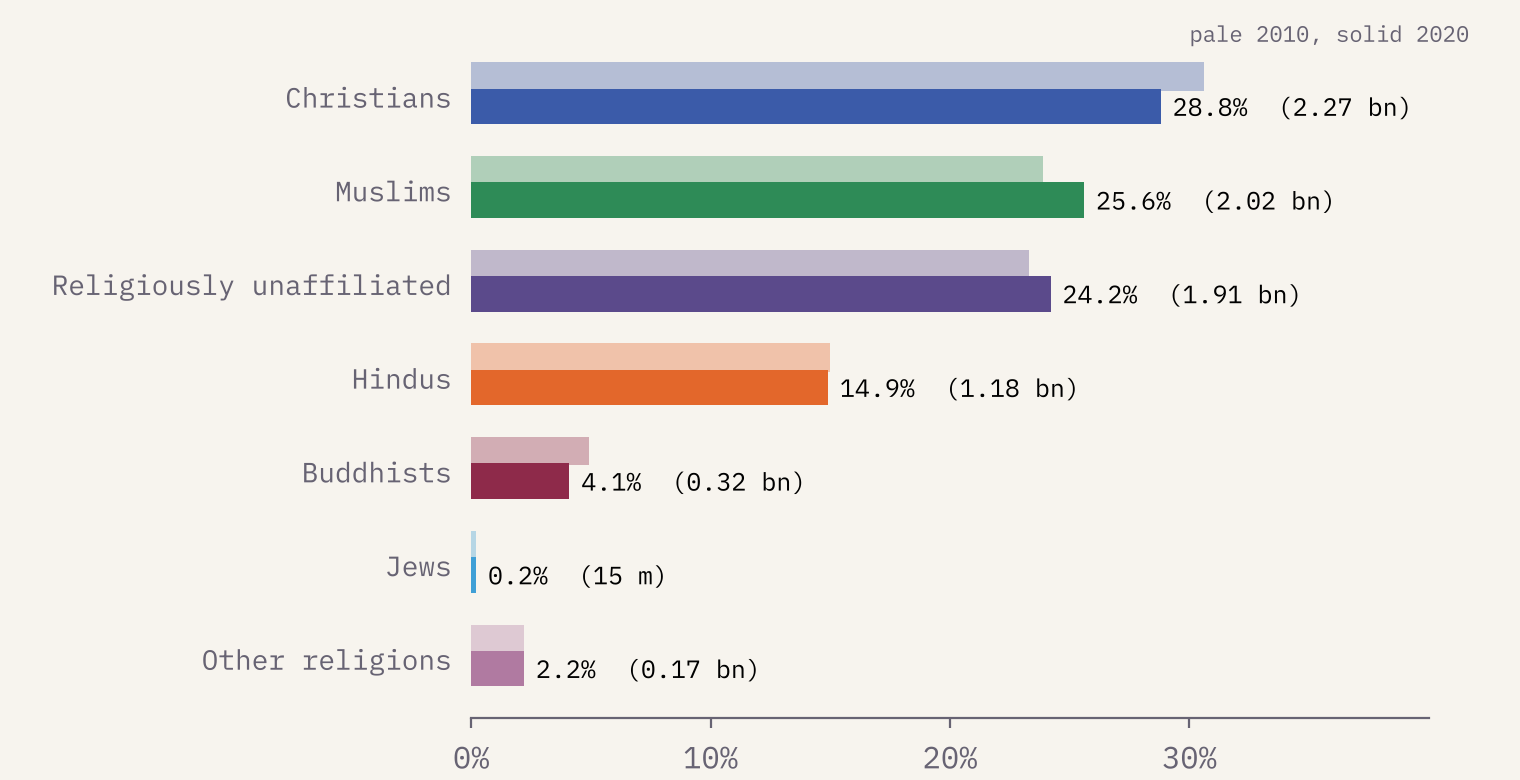
\includegraphics[width=.9\textwidth]{f_global.png}
\caption{The world's religious make-up in 2010 (pale) and 2020 (solid), with the number of people in 2020. Pew Research Center estimates.}\label{fig:global}\end{figure}

\begin{figure}[tbp]\centering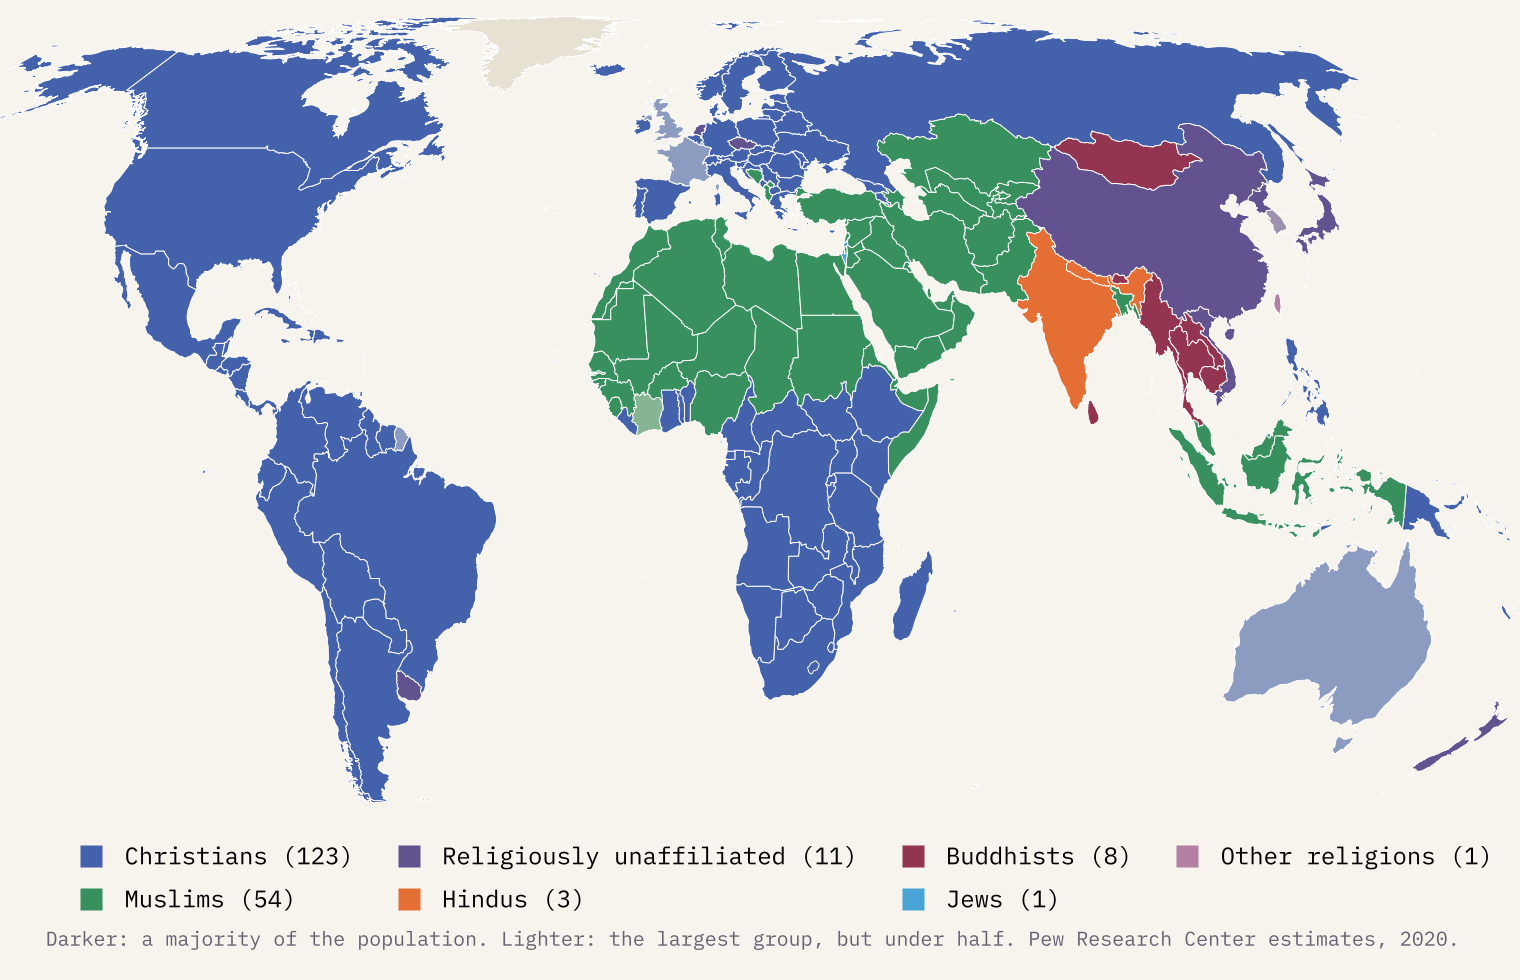
\includegraphics[width=\textwidth]{f_largest_map.png}
\caption{Largest religious group by country and territory, 2020. Darker shades mark a majority. Counts of countries in brackets.}\label{fig:largest}\end{figure}

\subsection{Change between 2010 and 2020}
The world's population grew by 12.3\%. Muslims grew fastest (20.7\%, 347 million), followed by the unaffiliated (16.5\%), Hindus (12.0\%), other religions (11.7\%), Jews (6.3\%) and Christians (5.7\%); the number of Buddhists fell by 5.4\%. The Christian share fell in 127 countries and territories and the unaffiliated share rose in 103. The largest rises in the unaffiliated share were in Australia (17.5 points), Chile (16.7), Uruguay (16.1) and the United States (13.3) (Figure~\ref{fig:nonechange}); in Uruguay and New Zealand the unaffiliated became the largest group. The share of Buddhists fell most in South Korea (-6.6 points) and Japan (-4.6).

The regional distribution of Christians shifted south (Figure~\ref{fig:christreg}). Sub-Saharan Africa's share of the world's Christians rose from 24.8\% to 30.7\% (532 to 697 million) and Europe's fell from 25.8\% to 22.3\% (554 to 505 million), so that by 2020 sub-Saharan Africa was home to more Christians than any other region.

\begin{figure}[tbp]\centering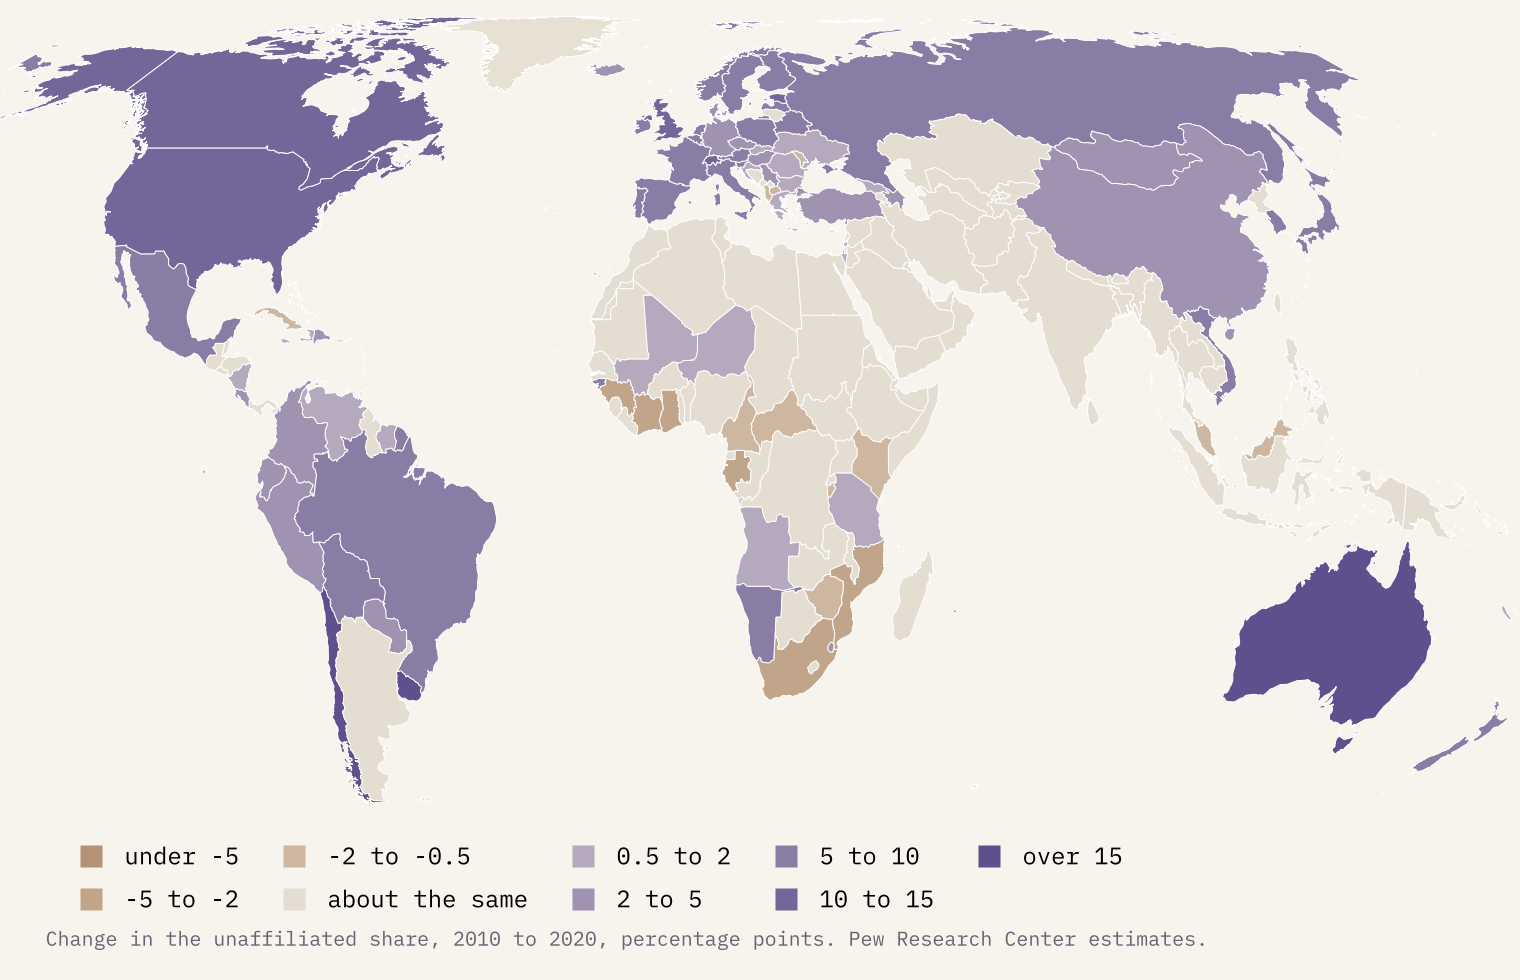
\includegraphics[width=\textwidth]{f_none_change_map.png}
\caption{Change in the share of people with no religious affiliation, 2010 to 2020, percentage points.}\label{fig:nonechange}\end{figure}

\begin{figure}[tbp]\centering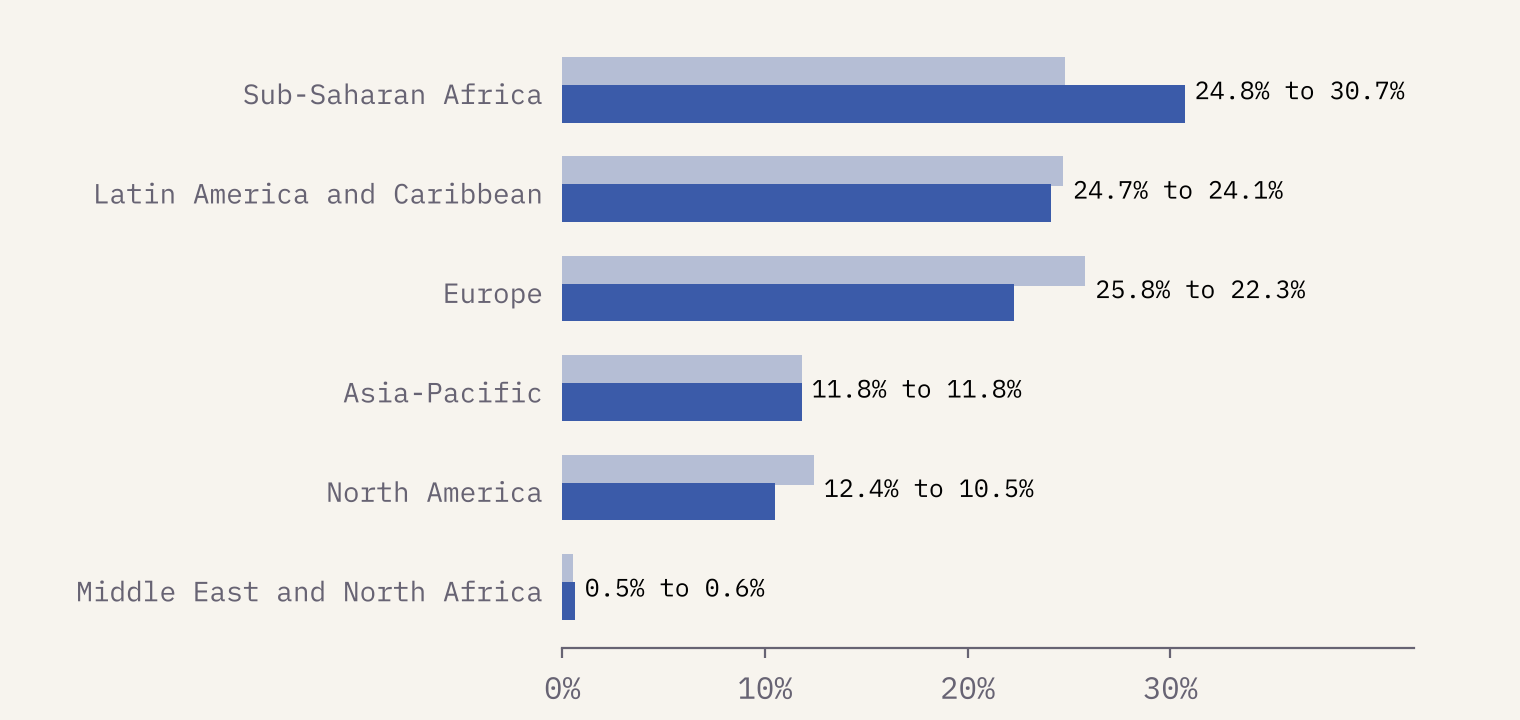
\includegraphics[width=.9\textwidth]{f_christ_regions.png}
\caption{Share of the world's Christians living in each region, 2010 (pale) and 2020 (solid).}\label{fig:christreg}\end{figure}

\subsection{Diversity}
On Pew's index the world as a whole scores 9.0 out of 10, but 41 countries and territories score very low and only 8 very high. The most diverse are Singapore (9.3), Suriname (7.5), Taiwan (7.5), South Korea (7.3) and Mauritius (7.3). Among regions, Asia-Pacific scores highest (8.7) and the Middle East and North Africa lowest (1.3).

\subsection{Places of worship in OpenStreetMap}
OpenStreetMap holds 1,624,818 places of worship: 989,563 tagged Christian, 291,813 Muslim, 111,463 Buddhist, 56,870 Hindu, 41,061 Shinto (99.4\% of them in Japan), 8,924 Taoist, 7,527 Jewish and 1,970 Sikh, with 106,390 (6.5\%) carrying no religion tag (Figure~\ref{fig:osm}). Only 64\% of Christian places carry a denomination tag. Among those that do (Figure~\ref{fig:den}), Catholic places make up 63.0\% in Europe and 61.2\% in Latin America and the Caribbean, where Pentecostal (9.5\%) and evangelical (7.6\%) churches follow. In North America, Baptist churches lead (32.6\%), then Catholic (13.8\%) and Methodist (12.7\%). In sub-Saharan Africa the largest tagged family is Orthodox (26.2\%), almost entirely in Ethiopia. In the United Kingdom the most tagged family is Anglican (16,952 of 38,818 Christian places).

Mapping is very uneven (Figure~\ref{fig:dens}). There are 77.5 mapped places of worship per 100,000 people in North America and 69.9 in Europe, against 11.6 in Asia-Pacific and 7.1 in sub-Saharan Africa. Per 100,000 Christians, North America has 114.6 mapped Christian places and sub-Saharan Africa 6.2. These differences reflect where volunteers map and how congregations meet as much as the number of buildings.

\begin{figure}[tbp]\centering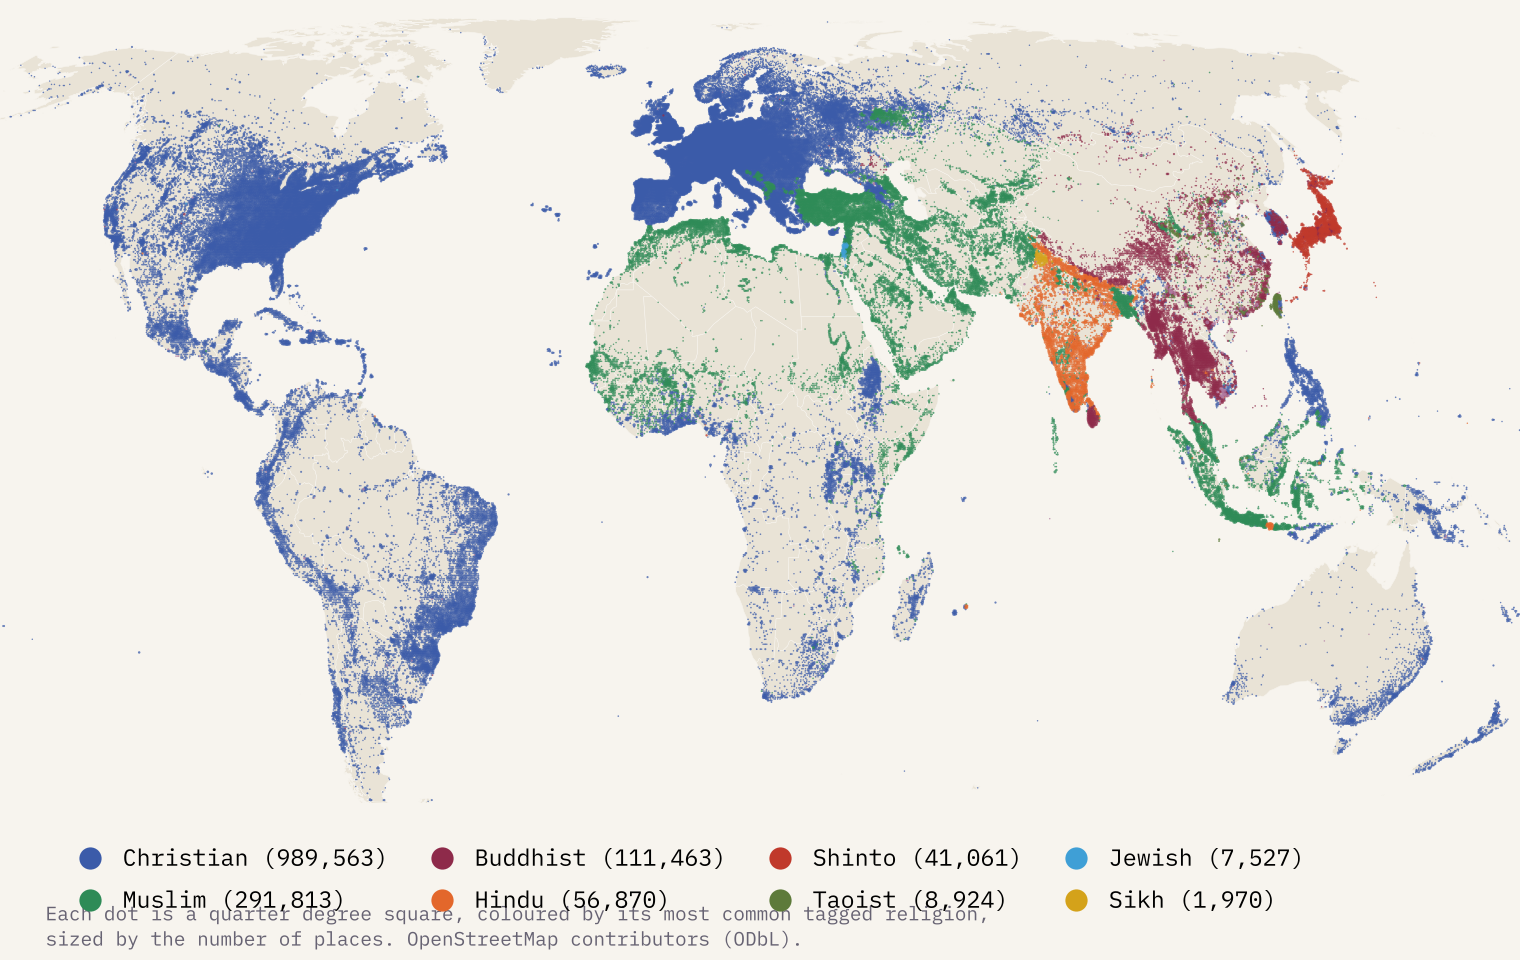
\includegraphics[width=\textwidth]{f_osm_map.png}
\caption{Places of worship in OpenStreetMap by quarter degree square, coloured by the most common tagged religion and sized by the number of places.}\label{fig:osm}\end{figure}

\begin{figure}[tbp]\centering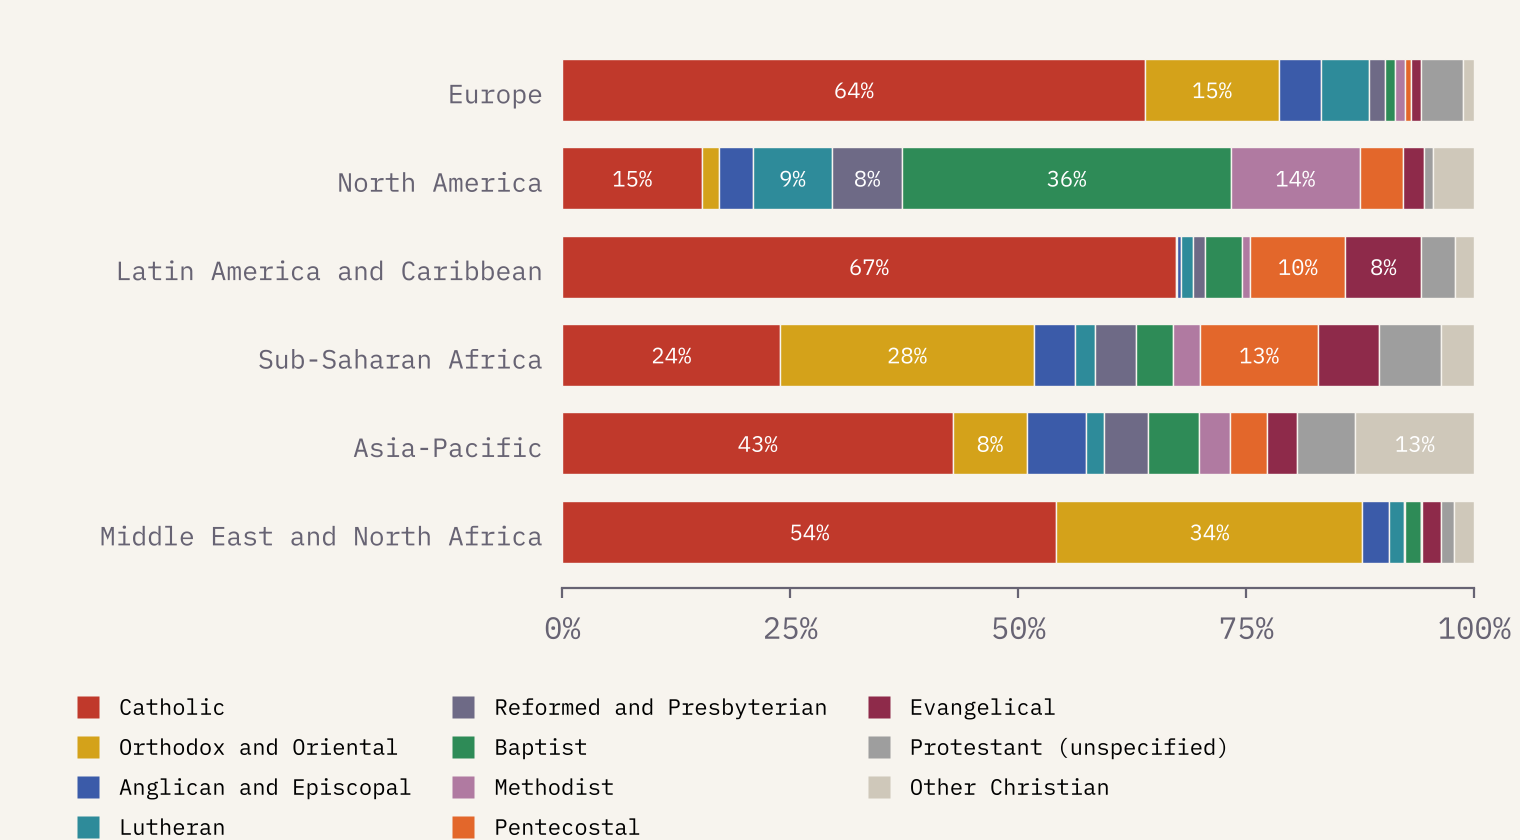
\includegraphics[width=.92\textwidth]{f_denominations.png}
\caption{Christian places of worship with a denomination tag, by denomination family and Pew region.}\label{fig:den}\end{figure}

\begin{figure}[tbp]\centering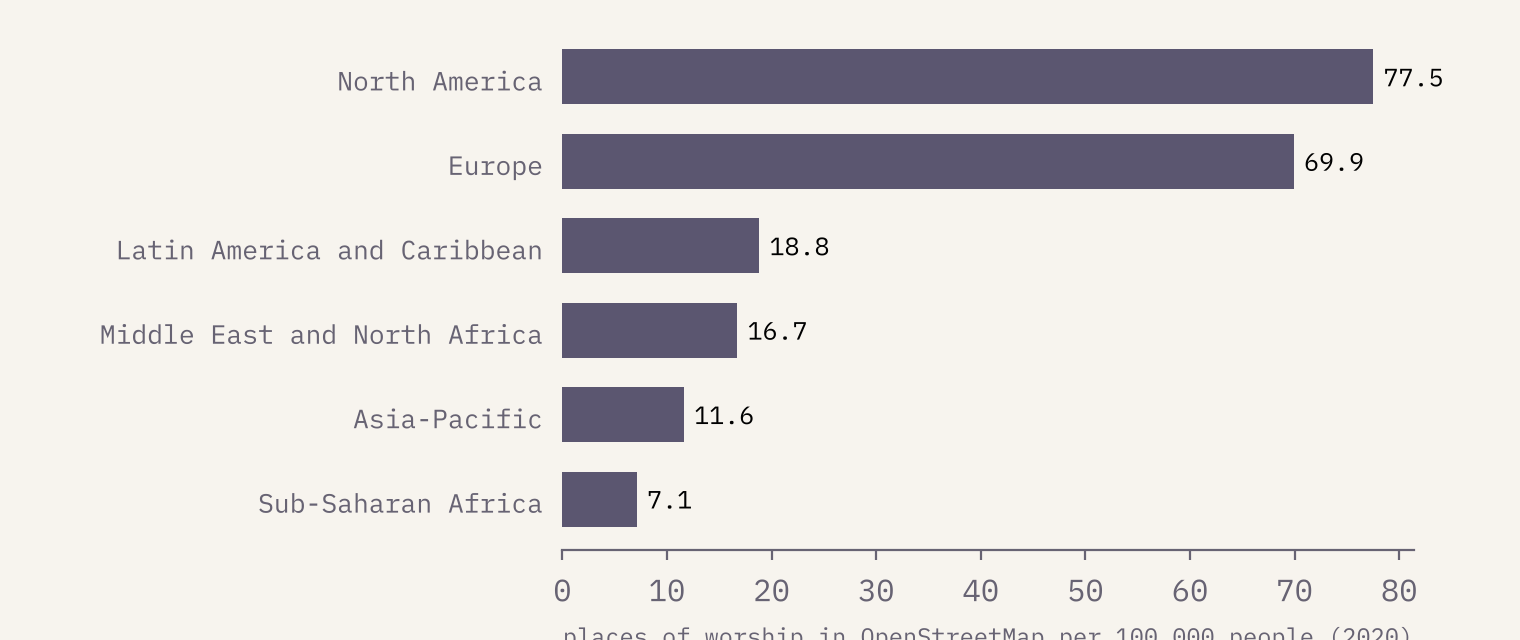
\includegraphics[width=.86\textwidth]{f_osm_density.png}
\caption{Places of worship mapped in OpenStreetMap per 100,000 people, by Pew region.}\label{fig:dens}\end{figure}

\subsection{The United Kingdom}
Table~\ref{tab:uk} and Figure~\ref{fig:nations} compare the four nations. In England and Wales, 46.2\% of usual residents were Christian in 2021 and 37.2\% had no religion, against 59.3\% and 25.1\% in 2011; the Muslim share rose from 4.8\% to 6.5\%. In Wales no religion is the largest answer (46.5\%), and in Scotland it is a majority (51.1\%), with 20.4\% Church of Scotland and 13.3\% Roman Catholic; no religion is a majority in 781 of Scotland's 1,279 intermediate zones. In Northern Ireland 79.7\% are Christian, 42.3\% Catholic and 37.4\% Protestant and other Christian, and 17.4\% have no religion. Across the three censuses together, 46.5\% of the UK's 66,940,560 counted residents were Christian and 37.8\% had no religion.

\begin{table}[tbp]\centering\small\caption{Religion in the UK nations, per cent of usual residents. England and Wales 2021, Scotland 2022, Northern Ireland 2021 (n/a: within other religion), and England and Wales 2011.}\label{tab:uk}\begin{tabular}{lrrrrr}\toprule & England & Wales & Scotland & N. Ireland & E and W 2011\\\midrule
Christian & 46.3 & 43.6 & 38.8 & 79.7 & 59.3\\
No religion & 36.7 & 46.5 & 51.1 & 17.4 & 25.1\\
Muslim & 6.7 & 2.2 & 2.2 & n/a & 4.8\\
Hindu & 1.8 & 0.4 & 0.6 & n/a & 1.5\\
Sikh & 0.9 & 0.1 & 0.2 & n/a & 0.8\\
Jewish & 0.5 & 0.1 & 0.1 & n/a & 0.5\\
Buddhist & 0.5 & 0.3 & 0.3 & n/a & 0.4\\
Other religion & 0.6 & 0.5 & 0.6 & 1.3 & 0.4\\
Not stated & 6.0 & 6.3 & 6.2 & 1.6 & 7.2\\
\bottomrule\end{tabular}\end{table}

\begin{figure}[tbp]\centering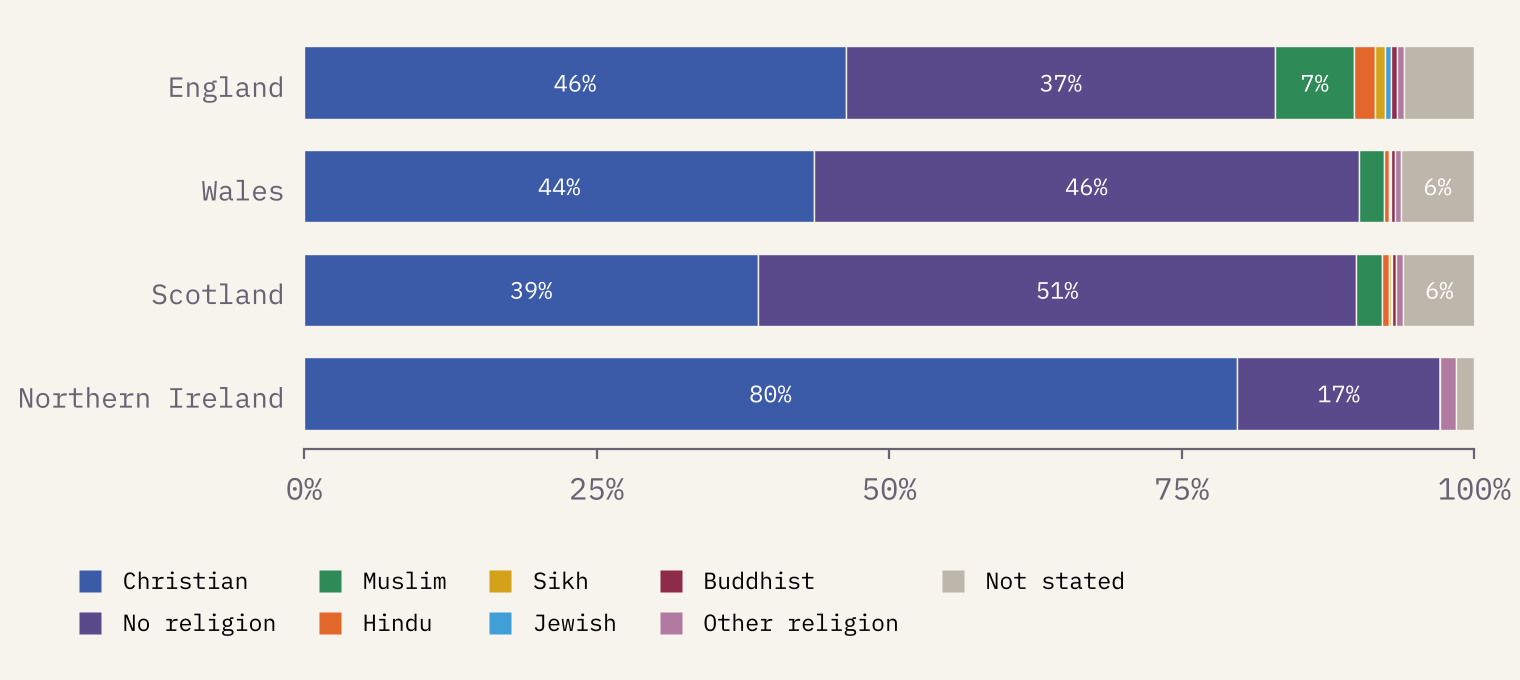
\includegraphics[width=.95\textwidth]{f_uk_nations.png}
\caption{Religion in the four UK nations (England and Wales 2021, Scotland 2022, Northern Ireland 2021). Northern Ireland's smaller faiths are within other religion.}\label{fig:nations}\end{figure}

No religion is the most common answer in 75 of the 361 local authorities (25 in Scotland, 11 in Wales, 39 in England), Muslim in two (Redbridge and Tower Hamlets) and Christian in the rest; in 2011 no religion was the most common answer in none of the councils of England and Wales. The Christian share fell in all 318 councils of England and Wales, by most in South Tyneside (-17.6 points) and least in Camden (-2.6). At neighbourhood level (Figure~\ref{fig:ukmap}), no religion is the most common answer in 1,599 of 7,264 MSOAs and Christian a majority in 2,772. The highest neighbourhood shares are 68.1\% no religion (Brighton and Hove 022), 75.6\% Christian (Liverpool 007), 87.0\% Muslim (Birmingham 070), 73.3\% Hindu (Leicester 010), 42.3\% Sikh (Ealing 044), 56.7\% Jewish (Salford 010) and 10.4\% Buddhist (Rushmoor 002). Among the detailed answers in England and Wales are 73,738 Pagan, 25,671 Alevi, 25,004 Jain, 12,820 Wicca and 9,583 Ravidassia.

\begin{figure}[tbp]\centering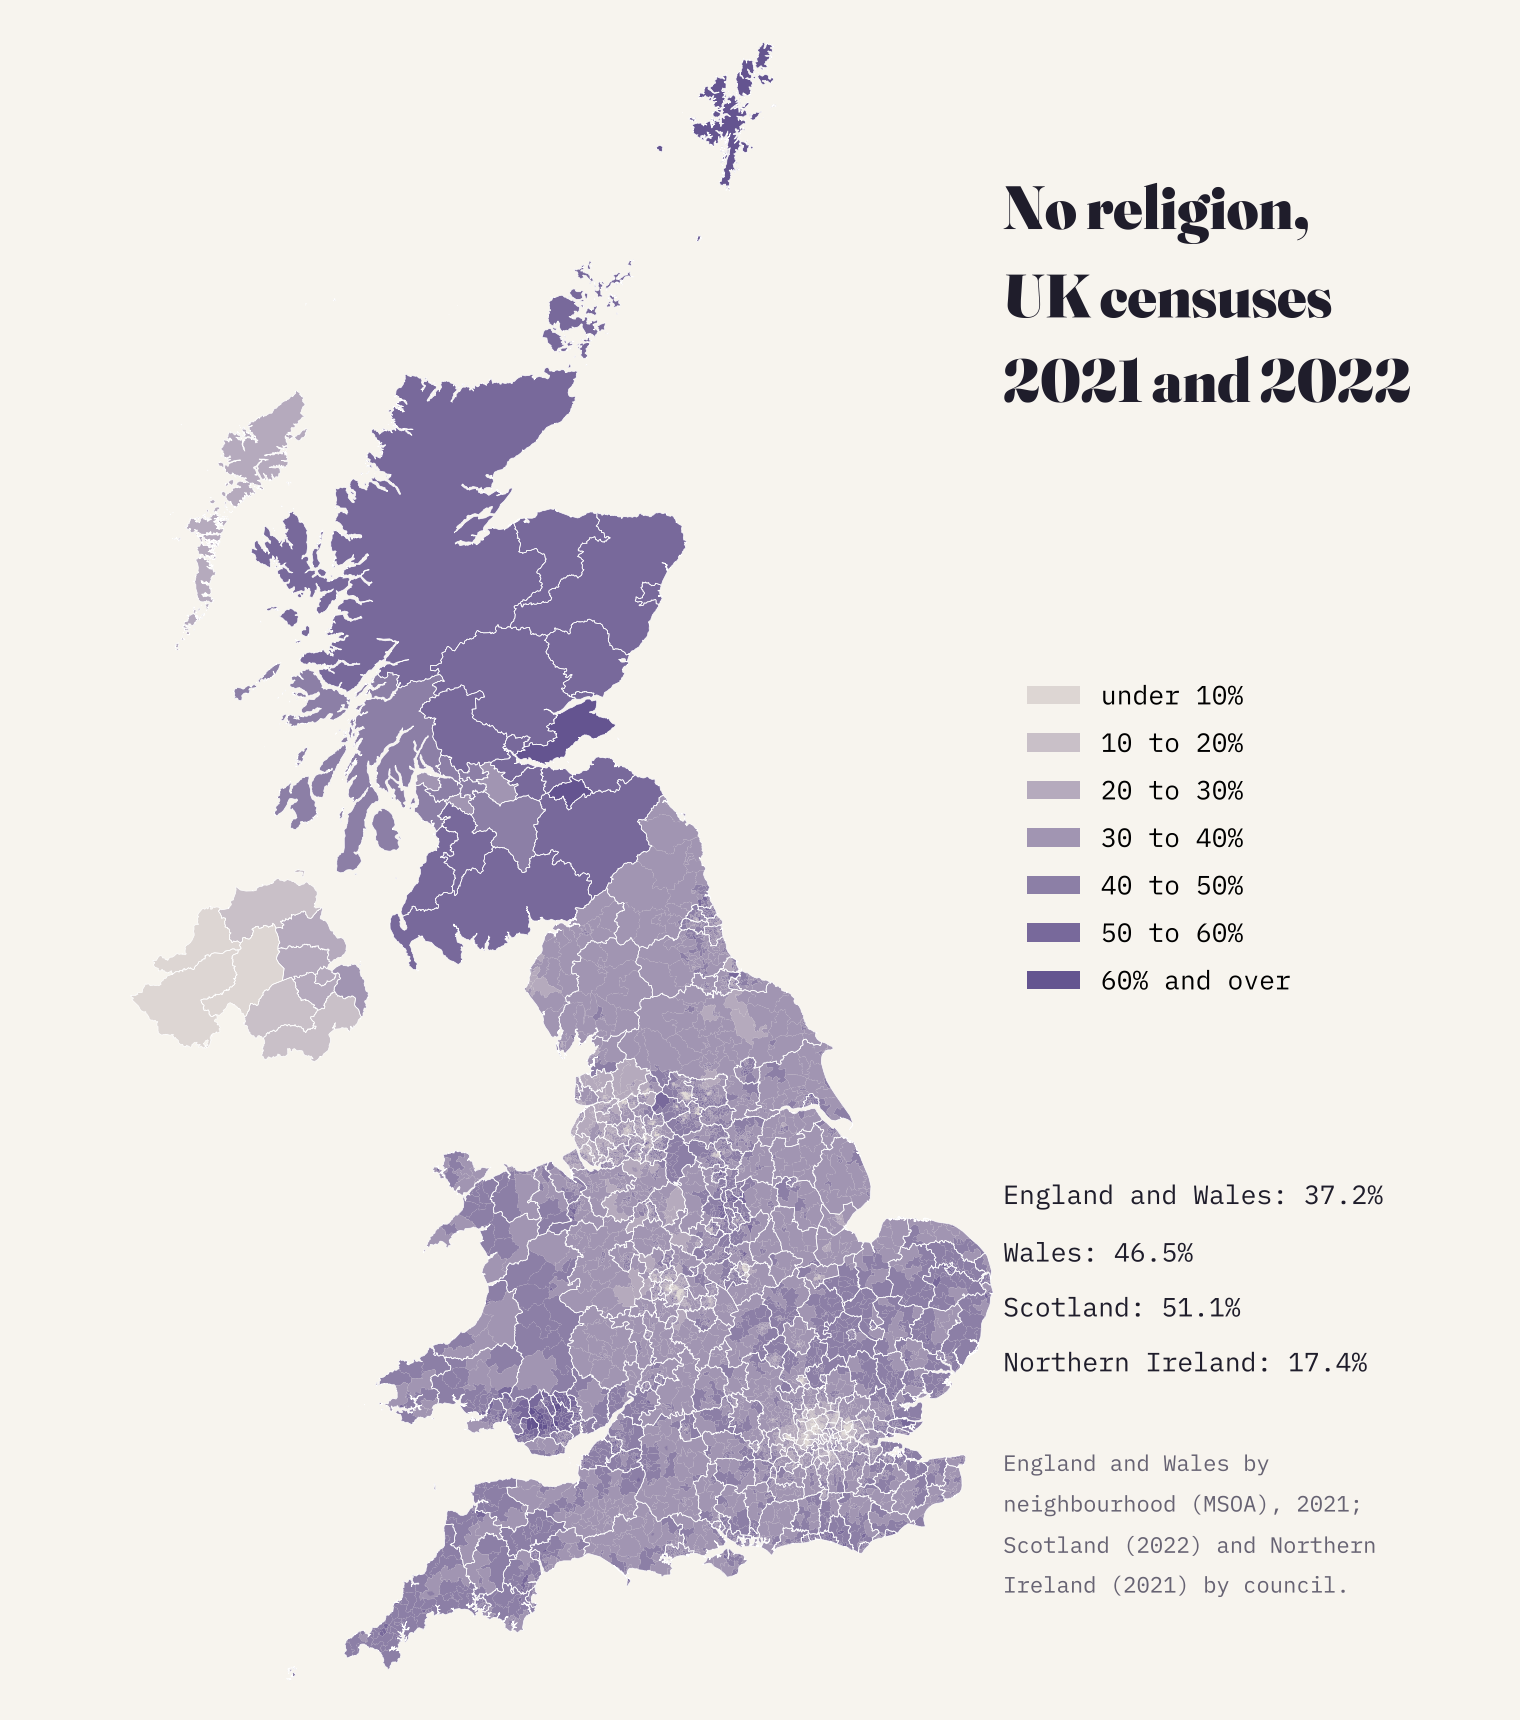
\includegraphics[width=.82\textwidth]{f_uk_none_map.png}
\caption{Share with no religion: England and Wales by MSOA (2021), Scotland (2022) and Northern Ireland (2021) by council. White lines are local authorities.}\label{fig:ukmap}\end{figure}

\subsection{Age}
Affiliation differs sharply by age (Figure~\ref{fig:age}). In England and Wales 76.7\% of people aged 75 and over were Christian and 13.6\% had no religion; among 25 to 34 year olds the figures were 31.2\% and 50.6\%, and the two are level among 35 to 49 year olds (40.6\% and 40.5\%). In Wales, 64.0\% of 25 to 34 year olds have no religion. The Muslim share is highest among under 16s (10.9\%) and lowest among those aged 75 and over (1.4\%).

\begin{figure}[tbp]\centering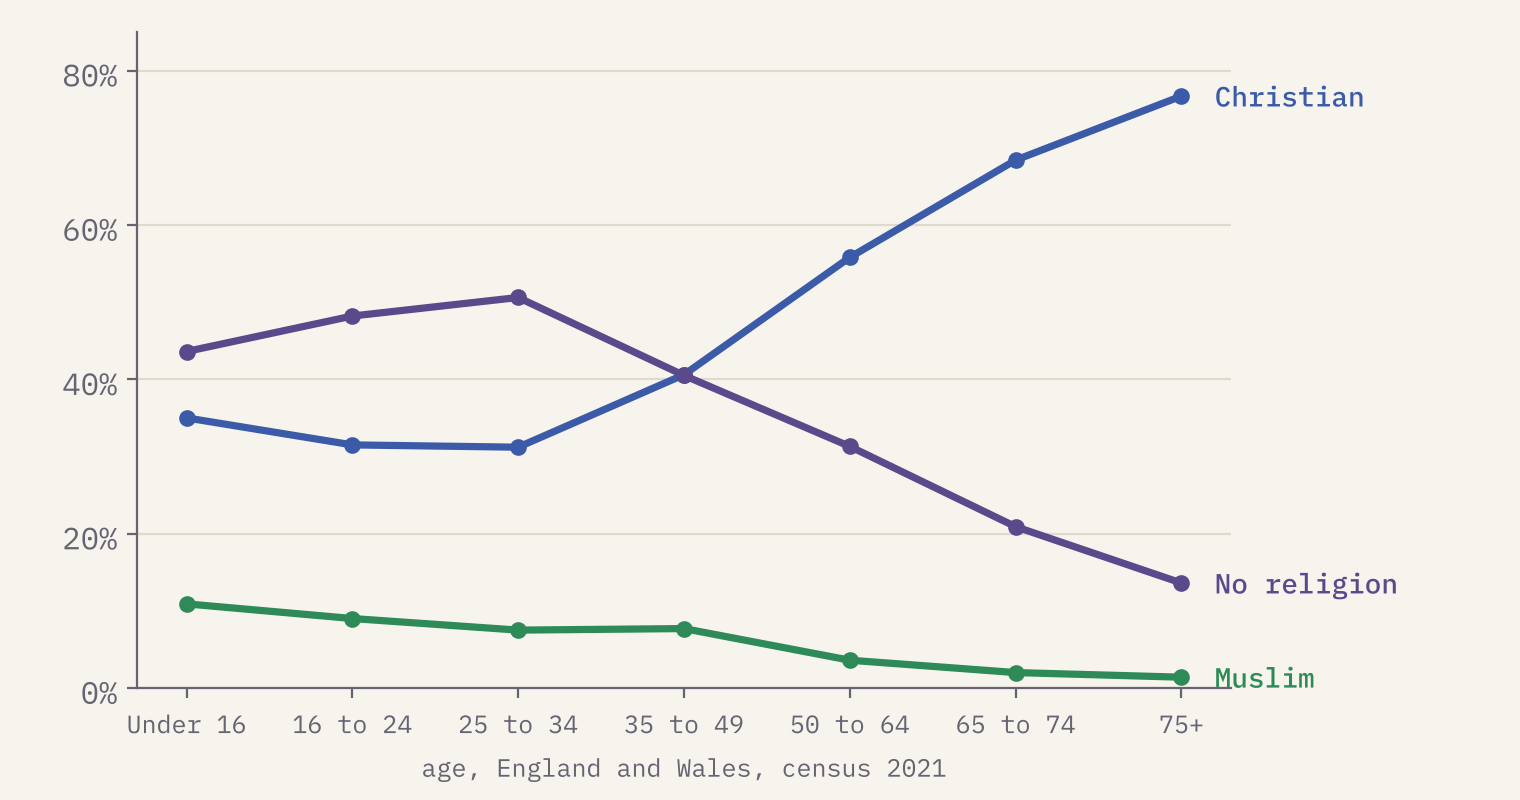
\includegraphics[width=.9\textwidth]{f_age.png}
\caption{Christian, no religion and Muslim shares by age, England and Wales, 2021.}\label{fig:age}\end{figure}

\subsection{Northern Ireland, 1861 to 2021}
Across 16 censuses (Figure~\ref{fig:ni}), the Catholic share was 40.9\% in 1861, fell to 28.0\% in 1981, a census affected by a campaign of non-cooperation and a high number not stating a religion, and rose to 42.3\% in 2021. The share belonging to the Presbyterian Church, the Church of Ireland and the Methodist Church together was 57.7\% in 1861, peaked at 62.2\% in 1926 and was 30.5\% in 2021; Catholics have outnumbered these three churches combined since 2001. The share with no religion or not stating one rose from 1.9\% in 1961 to 19.0\% in 2021. Counting religion brought up in as well, 45.7\% had a Catholic background in 2021 and 43.5\% a Protestant or other Christian background.

\begin{figure}[tbp]\centering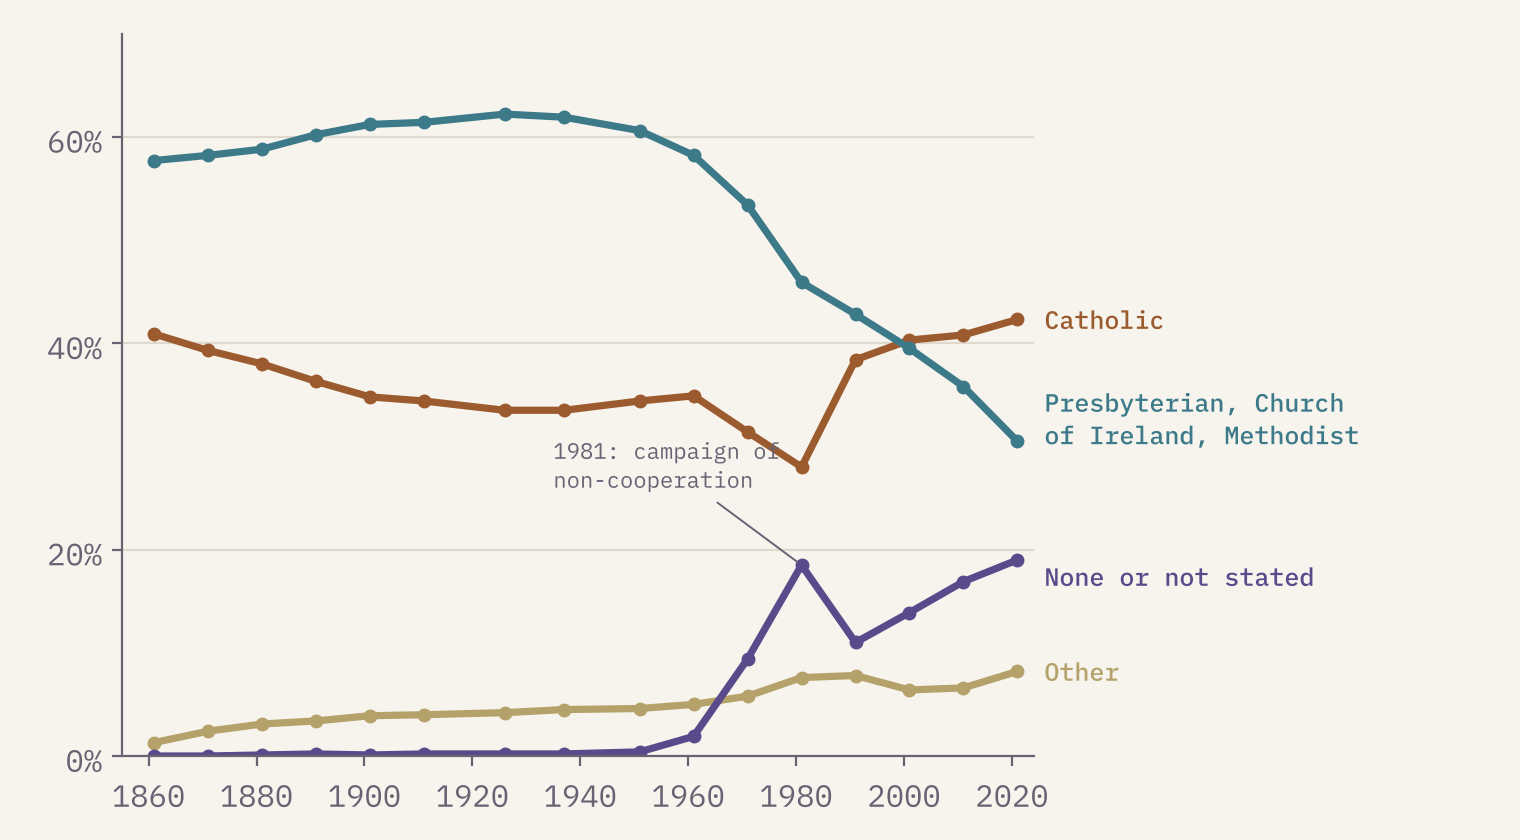
\includegraphics[width=.92\textwidth]{f_ni_history.png}
\caption{Religion in Northern Ireland at each census, 1861 to 2021 (current religion). Other includes smaller Protestant and other Christian denominations as well as other religions.}\label{fig:ni}\end{figure}

\section{Discussion}
The world picture is one of growth everywhere except among Buddhists, but of very different speeds. Muslim populations grew fastest, the unaffiliated grew faster than the world's population, and Christian numbers grew more slowly, so that the Christian share fell and the weight of world Christianity moved to sub-Saharan Africa. The largest rises in the unaffiliated share were in a group of mostly English-speaking and South American countries, while in several African countries, such as Mozambique, Ivory Coast and Ghana, it fell.

The UK censuses show the same movement away from affiliation in fine local detail, and they show how much of it is generational. The near mirror image between the oldest and the young adult age groups suggests that the national figures will continue to move as cohorts replace one another, although age patterns in a single census cannot by themselves separate the effect of age from that of generation. The local maps also show the concentration of minority faiths in particular towns and neighbourhoods, and the distinct position of Northern Ireland, where affiliation remains high and the long history of the Catholic and Protestant shares can be read from a single published series.

OpenStreetMap is a remarkable record of religious landscapes, but its gaps are large and patterned. It shows the parish churches of Europe and the United States in great detail and sub-Saharan Africa and much of Asia thinly, and only a minority of Christian places carry a denomination. It is best read alongside, not instead of, counts of people.

\section{Limitations}
First, affiliation is not belief or practice; none of the sources measures attendance or devotion. Second, Pew's figures are estimates, often projected from older censuses and surveys, and carry uncertainty that varies by country; the seven groups hide much variety, notably within other religions. Third, census answers depend on question wording, which differs between the UK nations and over time; Scotland's census was a year later, and Northern Ireland's tables do not separate smaller faiths. Fourth, the comparison between 2011 and 2021 uses 2023 council boundaries; small boundary changes other than mergers are ignored. Fifth, the age bands in the RM118 extract were identified from their totals rather than labels. Sixth, OpenStreetMap counts depend on volunteer mapping and tagging, which are very uneven, and quarter degree squares near borders and coasts may be assigned to the wrong country. Finally, all counts are for one retrieval date.

\section{Conclusion}
Open data can map religious affiliation from the world to the neighbourhood. Around the world, the decade to 2020 saw fast Muslim growth, a growing unaffiliated population and the movement of Christianity's centre to sub-Saharan Africa. In the UK, no religion has become the most common answer in Scotland, Wales and a fifth of councils, driven above all by the young. The atlas lets readers explore these patterns and, through the places of worship layer, see both religious landscapes and the limits of the open map.

\section*{Data and code availability}
The interactive atlas is at \url{https://maps.tristanhotham.com/religion-map/}. Data and code are at \url{https://github.com/Tristan-Hotham/religion-map} and archived with this paper at \url{https://doi.org/10.5281/zenodo.23842991}. Derived data are released under CC BY 4.0 (OpenStreetMap counts under the ODbL 1.0; census data contain public sector information under the Open Government Licence v3.0) and code under the MIT licence. Pew Research Center data are used with attribution and are available from Pew Research Center.

\section*{AI statement}
I wrote the text, with drafting and editing assistance from Claude (Anthropic), which also helped prepare the analysis code. I reviewed and checked all text and results.

\begin{thebibliography}{9}
\bibitem[Bast and Buchhold(2017)]{qlever} Bast, H. and Buchhold, B. (2017) QLever: a query engine for efficient SPARQL+text search. \emph{Proceedings of the 2017 ACM Conference on Information and Knowledge Management}, 647 to 656. \url{https://qlever.cs.uni-freiburg.de/}
\bibitem[Haklay and Weber(2008)]{osm} Haklay, M. and Weber, P. (2008) OpenStreetMap: user-generated street maps. \emph{IEEE Pervasive Computing}, 7(4), 12 to 18. Data: OpenStreetMap contributors, ODbL 1.0, \url{https://www.openstreetmap.org/copyright}
\bibitem[National Records of Scotland(2024)]{nrs2022} National Records of Scotland (2024) Scotland's Census 2022, table UV205: Religion. Open Government Licence v3.0. \url{https://www.scotlandscensus.gov.uk/}
\bibitem[Natural Earth(2026)]{naturalearth} Natural Earth (2026) Admin 0 countries (1:50m) and populated places (1:10m). Public domain. \url{https://www.naturalearthdata.com/}
\bibitem[NISRA(2022)]{nisra2021} Northern Ireland Statistics and Research Agency (2022) Census 2021 tables MS-B19, MS-B22 and MS-B23. Open Government Licence v3.0. \url{https://www.nisra.gov.uk/statistics/census}
\bibitem[ONS(2013)]{ons2011} Office for National Statistics (2013) 2011 Census table KS209EW: Religion. Nomis. Open Government Licence v3.0. \url{https://www.nomisweb.co.uk/}
\bibitem[ONS(2023a)]{ons2021} Office for National Statistics (2023) Census 2021 tables TS030, TS031 and RM118. Nomis. Open Government Licence v3.0. \url{https://www.nomisweb.co.uk/}
\bibitem[ONS(2023b)]{onsgeo} Office for National Statistics (2023) Middle layer super output areas (2021) and local authority districts (December 2023) boundaries. Open Government Licence v3.0; contains OS data © Crown copyright and database right. \url{https://geoportal.statistics.gov.uk/}
\bibitem[Pew Research Center(2025)]{pew2025} Pew Research Center (2025) How the global religious landscape changed from 2010 to 2020. Report and dataset `Religious Composition 2010-2020'. \url{https://www.pewresearch.org/religion/}
\bibitem[Pew Research Center(2026)]{pew2026} Pew Research Center (2026) Religious diversity around the world. \url{https://www.pewresearch.org/religion/2026/02/12/religious-diversity-around-the-world}
\end{thebibliography}
\end{document}
